\documentclass[11pt,a4paper]{article}
\usepackage{acl2010}
\usepackage{times}
\usepackage{amsfonts}
\usepackage{amssymb}
 \usepackage{graphicx}
\usepackage{amsmath}
\usepackage{multirow}
\usepackage{comment}
\usepackage{enumerate}
\usepackage{latexsym}
%\setlength\titlebox{6.5cm}    % Expanding the titlebox

\title{Finding Cognate Groups using Phylogenies}

\author{}

\date{}

\begin{document}
\maketitle
\begin{abstract}
  A central problem in historical linguistics is the identification
  of related ``cognate'' words. We present a generative model to
  automatically find these cognate groups which follows the
  phylogenetic relationships between languages. Our model uses
  weighted transducers to represent distributions over unobserved
  forms as well as the transformations from ancestor word to daughter
  word. We also present a novel method for simplifying the complex
  automata created during inference to counteract the otherwise
  exponential growth of message sizes. We test our model on two
  datasets where we significantly outperform a baseline approach.
  Finally, we demonstrate that these automatically reconstituted
  groups can be used to faithfully reconstruct ancestral words.
\end{abstract}
\section{Introduction}

The crowning achievement of historical linguistics has long been
the Comparative Method \cite{ohala93phonetics}, by which linguists
take assembled cognate words derived from a common ancestor word
to deduce the phonological and morphological changes that explains
the differences between them. For example, (XXX need to find a good
example). Typically, the Comparative Method requires the linguist
to make qualitative judgments regarding the relative likelihood of
certain sound changes. Recently, statistical methods have been introduced to provide
greater robustness to the Comparative Method.
\cite{oakes00computer,bouchard07probabilistic,bouchard09improved}

 However, these methods typically assume that the cognate words are already
given. Unfortunately, this is not always an easy task, since the
underlying morphological and phonological changes can obscure
relationships between words. More difficult still are the spurious
relationships between words that by chance or do to linguistic
universals. For example, both Mandarin and English \textit{/mama/}
(XXX probably find a better example) are phonologically quite similar
and have identical meanings, though few if any linguists would posit
a link between the two languages. Some authors have attempted to
automatically detect cognate words
\cite{lowe94reconstruction,oakes00computer,Kondrak01identifyingcognates,mulloni07automatic},
though these methods typically work on language pairs rather than on language
families.

In this paper we present a new generative model for the automatic
reconstitution of cognate groups given a family tree of languages
and word lists from those languages. Each word is generated from
its parent word by means of automatically learned transformations
inspired by the methods developed by linguists for the comparative
method. We present an iterative algorithm using bipartite graph matching
to fit the model to data.

% This needs to be here to convince latex to put it on page 2. 
\begin{figure*}
  \centering
  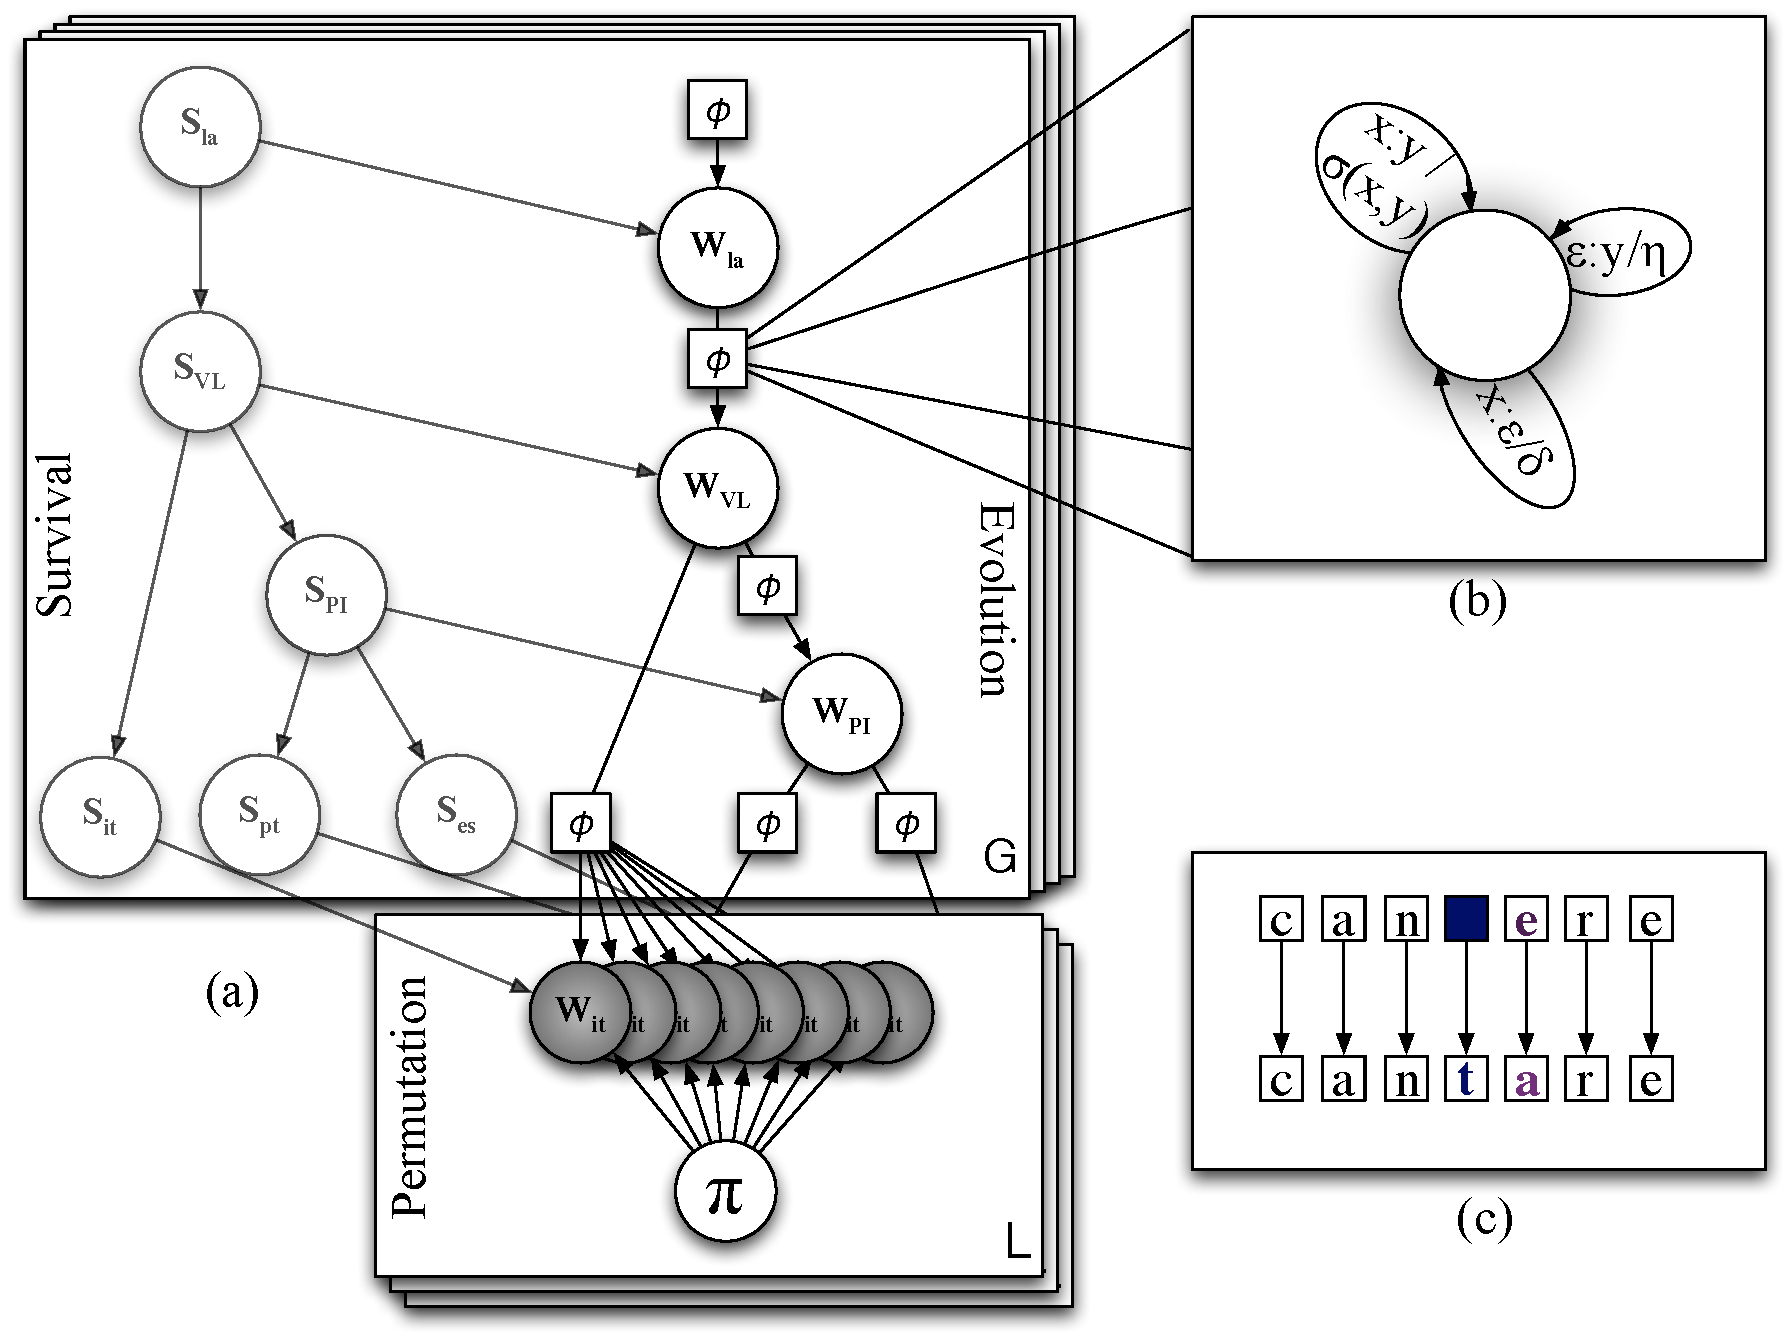
\includegraphics[scale=0.4]{gmodel}
  \caption{(a) The process by which cognate words are generated.
  Here, we show the derivation of Romance language words from their
  respective Latin ancestor. (b) The class of parameterized edit
  distances used in this paper. Each pair of characters has a weight
  $\sigma$ for deletion, and each character has weights $\eta$ and
  $\delta$ for insertion and deletion respectively. (c) A possible
  alignment produced by an edit distance.}
  \label{fig:gmodel}
\end{figure*}

Our model encodes distributions over strings as weighted finite
state automata. \cite{mohri09weighted} Weighted automata have been
successfully applied to speech processing \cite{Mohri96weightedautomata} and
more recently to morphology \cite{dreyer2009graphical}. We present
a new method for automatically compressing the automata that are
generated as messages during inference that can take into account
prior information about the expected outcome of inference.

In our experiments, we focus on two datasets. One is an automatically
transcribed word list of 584 cognate sets from three Romance languages
(Portuguese, Italian and Spanish), as well as their common ancestor
Latin. \cite{bouchard07probabilistic} The other is a hand-curated
list of nearly 60,000 cognates sets from 64 modern Austronesian
languages created by \newcite{blust93oceanic}. Both datasets are
transcribed into the International Phonetic Alphabet (Romance
automatically, Austronesian manually). 

One core difference between these datasets is that the Romance
dataset is dense while the Oceanic is sparse. Every cognate set in
the Romance dataset has a word for each language, while in the
Oceanic dataset only 1.6\% of possible slots are filled. Moreover,
it is entirely possible that the Oceanic dataset is incomplete:
there may be currently distinct cognate groups that are derived
from a single ancestral word!

(XXX one more short paragraph here?)

\section{Model}

In this section we describe a generative model for vocabulary lists
in multiple related languages given the phylogenetic relationship
between the languages (that is, their family tree). The generative
process falls into three subprocesses: survival, evolution, and
permutation. Survival dictates, for each cognate group, which
languages have words in that group. Evolution describes the process
by which words are transformed from their parent word. Finally,
permutation describes the ``scrambling'' of the word lists into an
order that bears no relation to their lineage. Each process is
described graphically in Figure (\ref{fig:gmodel}a), and we present
each in detail in the following subsections.

\subsection{Survival}

For each cognate group, our generative process starts by selecting
an ancestral word from the root language. Then, at each level, the
word may either die, and not spread to any of its children, or it
can continue. This process is modeled in a ``death tree'' with
variables $S_\ell$ specifying whether or not the word died before
reaching that language. Death at any node in the tree requires that
all of that node's descendants also be dead. This tree models the
intuition that a word is more likely to be found in two sibling
languages (e.g. Spanish and Portuguese) than in two cousin languages
(Portuguese and Italian) but not an intervening sibling
(Spanish). 

(XXX where to put this:) Also, because we do not know how many
cognate groups there may be ahead of time, we place a geometric
prior on the number of unobserved groups. (XXX)

\subsection{Evolution}

Once we know which languages will have an attested word and which
will not, we must generate the words. The evolution component of
the model generates words according to a transformation from their
immediate ancestor. The figure graphically describes our generative
model for three Romance languages: Italian, Portuguese, and Spanish.
In each cognate group, each word $W_\ell$ is generated from its
parent according to a conditional distribution with parameter $\phi$,
which is specific to that edge in the tree, but shared between all
cognate groups.

In this paper, $\phi$ takes the form of a parameterized edit distance
similar to the standard Levenshtein distance, though arbitrary
models--such as that in \newcite{bouchard07probabilistic}--could
be used. These transducers are represented schematically in Figure
(\ref{fig:gmodel}b). Characters $x$ and $y$ are arbitrary characters,
and $\sigma(x,y)$ represents the cost of substituting $x$ with $y$.
$\epsilon$ represents the empty character and is used as short hand
for insertion and deletion, which have parameters $\eta$ and $\delta$,
respectively.

As an example, see the illustration in Figure (\ref{fig:gmodel}c).
Here, the Vulgar Latin word \textit{cantare} is generated from its
parent form \textit{canere} by a series of edits: 4 matches, 1
substitution (from `e' to `a') and one insertion (the letter `t').
The probability of each individual edit is determined by $\phi$,
and the probability of the child Vulgar Latin word conditioned on
the Latin word is the sum over all possible alignments that generate
it.

\subsection{Permutation}

Finally, at the leaves of the trees are the observed words. (We
take interior nodes to be unobserved.) Here, we make the (false,
but simplifying) assumption that in any language there is at most
one word per language per cognate group. Because the assignments
of words to cognates is unknown, we specify an unknown parameter
$\pi_\ell$ for each language that specifies a permutation of the
words which specifies the mapping. From a generative perspective,
$\pi_\ell$ generates observed positions of the words in some
vocabulary list.

In this paper, our task is primarily to learn the permutations
$\pi_\ell$. All other hidden variables are auxiliary.

\section{Inference}

We are given a set of languages and a list of words in each language,
and our objective is to determine which words are cognate with each
other words. In the Romance dataset, we have the additional constraint
that each cognate group supports exactly one word from each language,
while in the Austronesian dataset we have at most one word from each
language. In effect, the inference task is reduced to finding a
permutation of the respective word lists to maximize the log
probability of the observed words:
\begin{equation}
  \begin{split}
    \vec{\pi} = \arg\!\max_{\vec \pi} \sum_{g} \log p(\vec w_{(\ell,\pi_\ell(g))}|\vec \phi,\vec \pi)
   \end{split}
 \end{equation}
Maximizing this equation directly is intractable, and so instead
we use a coordinate ascent algorithm to iteratively maximize one
permutation while holding the others fixed:
\begin{equation}
  \begin{split}
    \pi_\ell = \arg\!\max_{\pi_\ell} \sum_{g} \log p(\vec w_{(\ell,\pi_\ell(g))}|\vec \phi,\vec \pi_{-\ell},\pi_\ell)
  \end{split}
\end{equation}
Each iteration is then actually an instance of bipartite graph
matching, with the words in one language one set of nodes, and the
current cognate groups in the other languages the other set of
nodes, and the edge affinities between these nodes are the conditional
probability of each word belonging to each cognate group.

To compute the affinities for each cognate group, inference in each
tree computes the marginal distribution of the words from the ``held
out'' language. For the marginals, we use an analog of the 
forward/backward (XXX cite someone?) algorithm. In the upward pass,
we send messages from the leaves of the tree towards the root. For observed
leaf nodes $W_d$, we have:
\begin{equation*}
  \begin{split}
    \mu_{d\to a}(w_a) = \sum_{w_d} p(w_d|w_a,\phi)
   \end{split}
 \end{equation*}
and for interior nodes $W_i$:
\begin{equation*}
  \begin{split}
    \mu_{i\to a}(w_a) = \sum_{w_i} p(w_i|w_a) \prod_{d \in \mathrm{child}(w_i)} \mu_{d \to i}(w_i) 
  \end{split}
\end{equation*}
In the downward pass (toward the held-out language), we sum over ancestors word $W_a$:
\begin{equation*}
  \begin{split}
    \mu_{a\to d}(w_d) = \sum_{w_a} p(w_d|w_a) \prod_{\stackrel{d' \in \mathrm{child}(w_a)}{d' \neq d}} \mu_{d' \to a}(w_a) 
  \end{split}
\end{equation*}
Computing these messages recursively gives a marginal distribution
over the held-out language, and so we compute, for each word, the
probability of that word being in that cognate group. We then use
the Kuhn-Munkres algorithm \cite{Kuhn1955} to find the optimal
assignment for the bipartite matching problem, using the conditional
probabilities as inputs.

One important final note is initialization. In our early experiments
we found that choosing a random starting configuration usually led
to rather poor local optima. Instead, we started with empty trees,
and added in one language per iteration until all languages were
added, and then continued iterations on the full tree.

\section{Learning} 

So far we've only addressed learning the permutations $\pi$. However,
we also have two other sets of parameters: the transducers $\phi$,
and the death probabilities $S$. The parameters can be learned
through standard maximum likelihood estimation, which we detail in
this section.

Estimating the parameters for each survival parameter $S_\ell$ is
straightforward. Because we enforce that a word must be dead if its
parent word is dead, we just need to learn the conditional probabilities
$p($death$|$parent not dead$)$. Given fixed assignments $\pi$, we
simply count the number of ``deaths'' that occurred under a live
parent, apply smoothing--we found adding 0.5 to be reasonable--and
divide by the total number of live parents.

For the edit transducers $\phi$, we learn parameterized edit distances
which are essentially Levenshtein distances with a non-uniform
substitution, insertion, and deletion matrix, which we call
$\sigma(x,y)$ (XXX awkward relative clause). These edit distances
define a conditional exponential family distribution when conditioned
on an ancestral word (or when multiplied by a prior distribution
over those words). To construct the transducers, we first calculate
the marginal distribution over the edges connecting any two languages
$a$ and $d$. With this distribution, we the expected
``alignment unigrams.'' That is, we
need to compute for each pair of characters $x$ and $y$ the quantity:
\begin{equation}
  \begin{split}
    E_{p(w_a,w_d)}&[\#(x,y)] \\ = \sum_{w_a,w_d} &\sum_{\stackrel{z\in}{\scriptscriptstyle\mathrm{align(w_a,w_d)}}} \#(x,y) p(z|w_a,w_d)p(w_a,w_d)
   \end{split}
 \end{equation}
, where we denote $\#(x,y)$ to be the number of times the pair of characters
appears in the pair of strings, and $\mathrm{align}(w_a,w_d)$ is the set of possible
alignments between words $w_a$ and $w_d$. The exact method for computing
these counts is to use an expectation semiring introduced by
\newcite{eisner2001expectation}.

Given the expected counts, we now need to normalize them to ensure
that the transducer represents a conditional probability distribution.
Based on the derivation by \newcite{Oncina20061575}, we have that,
for each character $x$ in the ancestor language:
\begin{equation}
  \begin{split}
    \sum_{y \in \Sigma \cup \{\epsilon\}} \sigma(x,y) &= 1 - \sum_{y \in \Sigma} \sigma(\epsilon,y) \\
    \sigma(x,y) &\propto \frac{E[\#(x,y)]}{E[\#(x,\cdot)]} \\
    \sigma(\epsilon,y) &= \frac{E[\#(\epsilon,y)]}{E[\#(\cdot,\cdot)]} \\
   \end{split}
 \end{equation}
These equations ensure that the three transition types (substitution/match,
deletion, and insertion) are normalized for any ancestral character.

\section{Transducers and Approximations}

The procedure described in the preceding section would be quite
straightforward if the words $W$ were treated as indices into some
word list. Instead, in our model words are complex string-valued
random variables. To represent distributions and messages over these
variables, we chose weighted finite state automata, which can
compactly represent functions over strings. Unfortunately, while
initially compact, these automata can become unwieldy in inference,
and so approximations must be used.

In this section, we summarize the algorithms and representations
used for weighted finite state transducers.\footnote{For more
detailed treatment, we direct readers to \newcite{mohri09weighted}.}
We also describe a new procedure for approximating automata in a
message-passing environment.

\subsection{Weighted Automata}

Informally, a weighted automaton encodes a distribution over strings
(or pairs of strings) as weighted paths through a directed graph.
Each edge in the graph has a label (a single character, or the empty
character) and a weight. The weight of a string is then the sum
of all paths through the graph that accept a string.

More specifically, a weighted transducer assigns weights from a set
$S$ to pairs of strings with characters in alphabets $\Sigma$ and
$S$. Each path through the transducer corresponds to an alignment
between two strings, with an associated score for that alignment.
The weights in S must satisfy the semiring axioms, namely that there
is an operation $\oplus$ (addition) with an identity element $\bar
0$, an operation $\otimes$ with identity $\bar 1$ that distributes
over $\oplus$, and $\forall s\in S, s\otimes \bar 0 = \bar 0 \otimes
s = \bar 0$. Examples of semirings include the nonnegative real
numbers, the logarithms of the nonnegative reals, and the nonnegative
real numbers with $\otimes = +$ and $\oplus = \max$. These semirings
correspond to probabilities, log probabilities, and the Viterbi
approximation to log probabilities.

\begin{comment}
Formally, a weighted transducer over pairs of strings and a semiring
$(S,\oplus,\otimes,\bar 0, \bar 1)$ is a tuple
$(\Sigma,S,Q,I,F,E,\lambda,\tau)$, where $\Sigma$ is the
``input'' alphabet, $S$ the ``output'' alphabet, $Q$ a set of
states, $I \subseteq Q$ a set of initial states, $F \subseteq Q$ a
set of final states, $E \subseteq (Q \times Q \times (\Sigma \cup
\{\epsilon\}) \times (S\cup \{\epsilon\}) \times S)$ the set
of labeled and weighted edges, $\lambda: I \rightarrow S$ an initial
weight function, and $\tau: F \rightarrow S$ the final weight
function. ($\epsilon$ is a privileged ``null'' character character.)
A weighted acceptor can be viewed as a transducer over a single
alphabet, where the input and output labels are always the same
thing.
\end{comment}

In our setting, we are primarily concerned with transducers and
acceptors over the log semiring. In this case, a transducer assigns
a log-score to pairs of strings, and an acceptor similarly assigns
log-scores to single strings. These scores may or may not be
log probabilities.

\subsection{Transducer Operations}

For our purposes we are concerned with three fundamental operations
on weighted transducers. The first is computing the sum of all paths through a
transducer, which corresponds to computing the partition function
of a distribution. This operation can be performed in worst case
cubic time (using a generalization of the Floyd-Warshall Algorithm),
though for acyclic or feed-forward transducers this can be improved
dramatically by using a generalization of Djisktra's algorithm, the
Bellman-Ford algorithm or other related algorithms.

The second operation is the composition of two transducers. Intuitively,
composition creates a new transducer that takes the output from one
automata, processes it through the other transducer, and then returns
the output of that transducer. That is, consider two transducers
$T_1$ and $T_2$. $T_1$ has input alphabet $\Sigma$ and output
alphabet $S$, while $T_2$ has input alphabet $S$ and
output alphabet $\Omega$. The composition $T_1 \circ T_2$ returns
a new transducer over $\Sigma$ and $\Omega$ such that $(T_1 \circ
T_2)(s,t) = \bigoplus_{u} T_1(s,u)\otimes T_2(u,t)$. In this paper,
we use composition for marginalization. Given a factor $f_1(s,u;T_1)$
and another factor $f_2(u,t;T_2)$, composition corresponds to the
operation $\psi(s,t) = \sum_u f_1(s,u) f_2(u,t)$.

The third operation is transducer minimization. Transducer compositions
produces $O(nm)$ states, where $n$ and $m$ are the number of states
in each transducer. Repeated compositions compound the problem:
iterated composition of $k$ transducers produces $O(n^k)$ states.
Minimization alleviates this problem by collapsing indistinguishable
states into a single state. Unfortunately, minimization does not
always collapse enough states. In Section \ref{sec:approx}, we discuss approaches
to ``lossy'' minimization that produce automata that are not exactly
the same but are typically much smaller.

\subsection{Message Approximation}
\label{sec:approx}

Unfortunately, the maximal number of states in a message in each
cognate group is exponential in the number of words assigned to
that group. Minimization can only help so much: in order for two
states to be collapsed, the distribution over transitions from those
states must be indistinguishable, or indistinguishable to within
some tolerance. In practice, for the kinds of transducers generated
in our model, minimization removes at most half the states, which
is not sufficient to counteract the exponential growth. Thus, we
need to find a way to approximate a message $\mu(x)$ by some simpler
distribution $\tilde\mu(x;\theta)$ that has some simpler form with
parameter $\theta$.

In the context of transducers, previous authors have focused on a
combination of n-best lists and unigram\footnote{Here, and for the
rest of the paper, the ``grams'' of interest are characters in the
International Phonetic Alphabet.} back-off models. \cite{dreyer2009graphical}
In our setting, n-best lists seem inadequate; early experiments
showed that a 10,000-best list for a typical message only accounts
for 50\% of message log perplexity. That is, the posterior marginals in
our model are (at least initially) fairly flat.

% Put this here to make it come before the section heading Message Topologies
\begin{figure*}
  \centering
  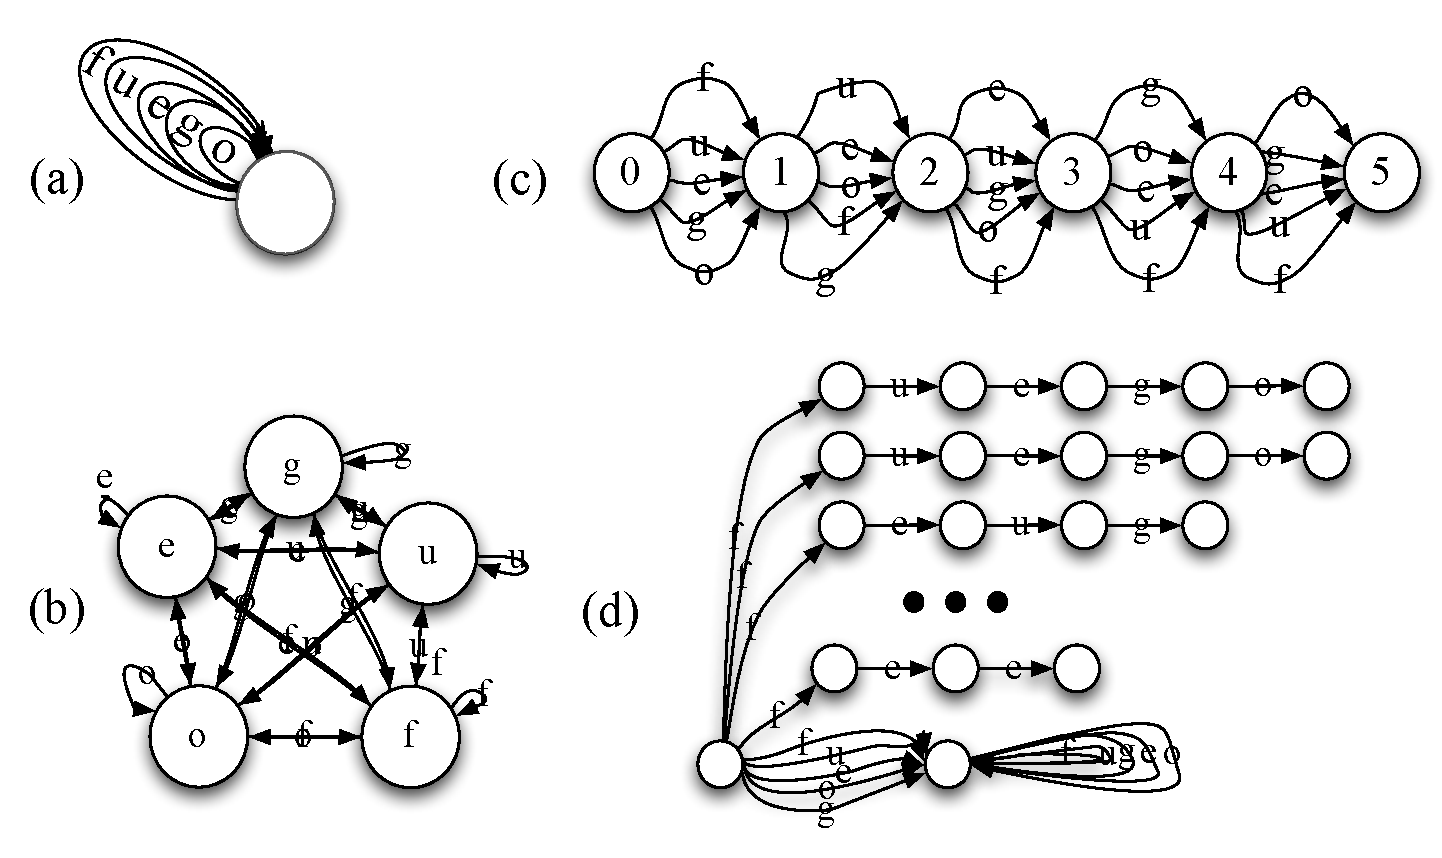
\includegraphics[scale=0.4]{fsa}
  \caption{Various topologies for approximating topologies: (a) a
  unigram model, (b) a bigram model, (c) the anchored unigram model,
  and (d) the kbest model plus backoff model used in
  \newcite{dreyer2009graphical}. In (c) and (d), the relative height
  of arcs is meant to convey approximate probabilities.}
  \label{fig:fsa}
\end{figure*}


An alternative approach might be to simply treat messages as
unnormalized probability distributions, and to minimize the KL
divergence between some approximating message and the true message.
However, messages are not always probability distributions and--because
the distribution over potential strings is in principle infinite--they
need not sum to a finite number. Instead, we propose to minimize
the KL divergence between the ``expected'' marginal distribution
and the approximated ``expected'' marginal distribution:
\begin{equation}
  \begin{split}
    \hat\theta &= \arg\!\min_{\theta} D_{KL}(\tau(w)\tilde\mu(w;\theta)||\tau(w)\mu(w) ) \\
    &= \arg\!\min_{\theta} \sum_w \tau(w) \tilde\mu(w;\theta) \log \frac{\tau(w)\tilde\mu(w;\theta)}{\tau(w)\mu(w)} \\
    &= \arg\!\min_{\theta} \sum_w \tau(w) \tilde\mu(w;\theta) \log \frac{\tilde\mu(w;\theta)}{\mu(w)} \\
   \end{split}
 \end{equation}
where $\tau$ is a prior distribution acting as a surrogate for the
posterior distribution over $w$ without the information from $\mu$.
That is, we seek to approximate $\mu$ not on its own, but as it
functions in an environment representing its final context.

In this paper, $\mu(w)$ is a complex automaton with potentially
many states, $\tilde\mu(w)$ is a simple parametric automaton with
forms that we discuss below, and $\tau(w)$ is an arbitrary (but
hopefully fairly simple) automaton. The actual method we use is as
follows. Given a deterministic prior transducer $\tau$, and a
deterministic automaton topology $\tilde\mu^*$, we created the
composed unweighted automaton $\tau \circ \tilde\mu^*$, and calculate
arc transitions weights to minimize the KL divergence between that
composed transducer and $\tau\circ\mu$. The procedure for calculating
these statistics was described in \newcite{li2009first}, which
amounts to using an expectation semiring \cite{eisner2001expectation}
to compute expected transitions in $\tau\circ\mu$.

From there, we need to created the transducer $\tau^{-1}
\circ\tau\circ\tilde\mu$. That is, we need to divide out the influence
of $\tau(w)$. Since we know the topology and arc weights for $\tau$
ahead of time, this is often as simple as dividing arc weights in
$\tau\circ\tilde\mu$ by the corresponding arc weight in $\tau(w)$.
For example, if $\tau$ encodes a geometric distribution over word
lengths and a uniform distribution over characters (that is, $\tau(w)
\propto {p^{|w|}}$), then computing $\tilde\mu$ is as simple as
dividing each arc in $\tau\circ\tilde\mu$ by $p$.\footnote{Actually,
we must be sure to divide each ``final weight'' in the transducer
by $(1-|\Sigma| p)$, which is the stopping probability for a geometric
transducer.}

There are a number of choices for $\tau$. One is a hard maximum on
the length of words; that is, one that assigns some uniform probability
to all strings of length K or less. Another is to choose $\tau(w)$
to be a unigram language model over the language in question with
a geometric probability over lengths. In our experiments, we find
that $\tau(w)$ can be a geometric distribution over lengths with a
uniform distribution over characters and still obtain reasonable
results.  This distribution captures the importance of shorter
strings while still maintaining a relatively weak prior.

\subsection{Message Topologies}

What remains is the selection of the topologies for the approximating
message $\tilde\mu$. We consider three possible approximations,
illustrated in Figure \ref{fig:fsa}. The first is a plain unigram
model, the second is a bigram model, and the third is an anchored
unigram topolgy: a position-specific unigram model for each position
up to some maximum length.

The standard unigram model has $|\Sigma|+2$ parameters:
one weight $\sigma_a$ for each character $a \in \Sigma$, a ``starting
weight'' $\lambda$, and a stopping probability. Estimating this
model involves only computing the expected count of each character,
along with the expected length of a word, $E[|w|]$. We then normalize
the counts according to the maximum likelihood estimate, which
gives: 
\begin{equation*}
  \begin{split}
    \sum_{a\in\Sigma} \sigma_a &= \frac{E[|w|]-1}{E[|w|} \\
    \sigma_a &\propto E[\#(a)]
   \end{split}
 \end{equation*}
with the stop probability taking the remaining mass. Recall that
these expectations can be computed using an expectation semiring.

$\lambda$ can be computed by ensuring that the
approximate and exact expected marginals have the same partition
function. That is, with the other parameters fixed solve:
\begin{equation*}
  \begin{split}
    \sum_w \tau(w) \tilde\mu(w) = \sum_w \tau(w) \mu(w)
  \end{split}
\end{equation*}

The second topology we consider is the bigram topology, which is
similar to the unigram topology except that instead of a single
state, we have a state for each character in $\Sigma$, along with
a special start state. Each state $a$ has transitions with weights
$\sigma_{b|a}= p(b|a)$. Normalization is straightforward:
\begin{equation*}
  \begin{split}
    \sum_{b\in\Sigma} \sigma_{b|a}&= 1-\sigma_{\mathrm{stop}|a} \\
    \sigma_{b|a} &\propto E[\#(b|a)]
   \end{split}
 \end{equation*}

The final topology we consider takes positional information into
account. Namely, for each position (up to some maximum position),
we have a unigram model over characters emitted at that position,
along with the probability of stopping at that position. Estimating
the parameters of this model is similar, except that the expected
counts for the characters in the alphabet are conditioned on their
position in the string. With the expected counts for each position,
we normalize each state's final and outgoing weights. In our
experiments, we typically set the maximum string length to 7 + the
longest observed string.

\section{Experiments}

We conduct three experiments. The first is a ``complete data''
experiment, in which we reconstitute the cognate groups from Romance
where we know that all cognate groups have words in all three
languages. The second is a ``partial data'' experiment, in which
we examine a subset of 10 languages in the Oceanic dataset. Here,
only a fraction of words appear in any cognate group. The third is
the task of proto-word reconstruction given these automatically
created groups. For reconstructions, we use the inference methods
from \newcite{bouchard09improved}.

As a baseline, we use a variant of our inference algorithm where
instead of automata we use Dice's coefficient, which is commonly
used in bilingual detection of cognates.
\cite{Kondrak01identifyingcognates,Kondrak03cognatescan} Dice's
coefficient is defined, for sets X and Y, as:
\begin{equation}
  \begin{split}
    DICE(X,Y) &= \frac{2 |X\cap Y|}{|X| + |Y|}
   \end{split}
 \end{equation}
We follow prior work and use sets of bigrams within words.  During
bipartite matching the set X is the set of bigrams in the held-out
language, and Y is the union of bigrams in the other languages.
When the number of congate groups is not known,
we XXX (not sure still\dots)

\subsection{Experiment 1: Complete Data}

In this experiment, we know precisely how many cognate groups there
are and that every cognate group has a word in each language. This
is, of course, an unrealistic scenario, but it represents a good
test case of how well these models can perform without the
non-parametric task of decided how many clusters to use.

We scrambled the 584 cognate groups in the Romance dataset and ran
the algorithm to convergence. Besides the baseline, we tried using
Unigrams, Anchored Unigrams, and Bigrams with and without learning
the parametric edit distances. When we didn't use learning, we set
the parameters of the edit distance to (0, -3, -4) for matches,
substitutions, and deletions/insertions, respectively. With learning
enabled, transducers were initialized with these parameters.

For evaluation, we report two metrics. The first is pairwise accuracy
for each pair of languages averaged across pairs. The other is
accuracy measured in terms of the number of correctly and completely
reconstructed cognate groups.

Table \ref{tbl:exp1} shows the results under various configurations. XXX

\begin{table*}
  \centering
  \begin{tabular}{|c|c|c|c|}
    Transducers & Messages & Pair Acc. & Rec. Acc.\\
    \hline
    N/A & Baseline & 48.1 & 35.4  \\
    \hline
    Levenshtein&Unigrams & 37.2 & 26.2 \\
    Levenshtein&Anchored Unigrams & 68.6 & 56.8\\
    Levenshtein&Bigrams & & \\
    \hline 
    Learned&Unigrams & & \\
    Learned&Anchored Unigrams & 90.3  & 86.6 \\
    Learned&Bigrams & & \\
  \end{tabular}
  \caption{Accuracies for reconstructing cognate groups. Levenshtein
  refers to fixed parameter edit distance transducer. Learned refers
  to automatically learned edit distances.}
  \label{tbl:exp1}
\end{table*}

\subsection{Experiment 2: Austronesian}

\subsection{Experiment 3: Reconstructions}


\begin{comment}
  (XXX this is mostly worked in, just leaving here for reference)
\section{Previous Work}

1) The reconstruction engine: a computer implementation of the
comparative method\\
  A deterministic approach from 1994 designed to help linguists look
at reconstructions. Closer to Alex's stuff. \\
2) Automatic Detection of Orthographic Cues for Cognate Recognition (2006) \\
  Given a list of english/german words (translations of each other),
are they cognate? Pretty crappy paper.\\
3) Identifying Cognates by Phonetic and Semantic Similarity \\
  The most similar. Given a list of multiple words from four Native
American languages, sort out which words are cognate. Uses their
English glosses to look up WordNet distance in addition to phonetic
distances. Phonetic distances are measured either using DICE on
bigrams, Longest Common Subsequence, and then a kind of edit distance
on phone classes (that was earlier work he borrowed. ALINE) *DICE on
bigrams and LCS look like good baselines.*\\
  -- This approach was geared towards precision/recall, and in some
sense is the real task. I'll see if I can find the data. \\
4)  Combining Evidence in Cognate Identification (2004) \\
  A very similar paper to (3). Uses ALINE to do phonetic comparisons.
Doesn't compute proto-projections like we do. Direct comparison of
words. Performance in the 50-65\% Average Precision range.\\
6) Semi-Supervised Learning of Partial Cognates using Bilingual Bootstrapping
  Basically context driven. Different task, but probably worth mentioning.
\end{comment}

\section{Conclusion}

XXX future work: talk about adding in semantics a la \newcite{Kondrak01identifyingcognates}, removing the
bipartite restriction, and joint reconstruction and reconstitution
\clearpage
\bibliographystyle{acl}
\bibliography{refs}


\end{document}
